% =======================================================
% 简易编译器设计指导手册
% 编译命令: xelatex 指导1.tex (需运行两次生成目录)
% 依赖: ctex, tikz, tcolorbox, listings 等常见宏包
% =======================================================
\documentclass[12pt, a4paper]{ctexart}

% -------------------------------------------------------
% 基础宏包
% -------------------------------------------------------
\usepackage{geometry}
\usepackage{xcolor}
\usepackage[colorlinks=true, linkcolor=NavyBlue, urlcolor=NavyBlue]{hyperref}
\usepackage{listings}
\usepackage{tikz}
\usetikzlibrary{arrows.meta, positioning, calc}
\usepackage{tcolorbox}
\tcbuselibrary{skins, breakable}
\usepackage{amsmath}
\usepackage{booktabs}
\usepackage{array}
\usepackage{enumitem}
\usepackage{fancyhdr}
\usepackage{titlesec}
\usepackage{multirow}

% -------------------------------------------------------
% 颜色定义
% -------------------------------------------------------
\definecolor{NavyBlue}{RGB}{0, 86, 150}
\definecolor{LightBlue}{RGB}{219, 234, 254}
\definecolor{CodeBg}{RGB}{248, 249, 250}
\definecolor{WarnBg}{RGB}{255, 243, 205}
\definecolor{TipBg}{RGB}{209, 236, 241}
\definecolor{KeyBg}{RGB}{255, 225, 225}
\definecolor{DarkGray}{RGB}{50, 50, 50}
\definecolor{CodeGreen}{RGB}{0, 128, 0}
\definecolor{CodePurple}{RGB}{128, 0, 128}

% -------------------------------------------------------
% 页面布局
% -------------------------------------------------------
\geometry{left=2.5cm, right=2.5cm, top=3cm, bottom=3cm}
\setlength{\parindent}{2em}
\setlength{\parskip}{4pt}

% -------------------------------------------------------
% 代码块样式
% -------------------------------------------------------
\lstset{
  backgroundcolor  = \color{CodeBg},
  basicstyle       = \small\ttfamily,
  breaklines       = true,
  breakatwhitespace= false,
  captionpos       = b,
  commentstyle     = \color{CodeGreen},
  keywordstyle     = \color{NavyBlue}\bfseries,
  stringstyle      = \color{CodePurple},
  numberstyle      = \tiny\color{gray},
  numbers          = left,
  numbersep        = 8pt,
  frame            = single,
  framerule        = 0.5pt,
  rulecolor        = \color{gray!30},
  tabsize          = 4,
  showspaces       = false,
  showstringspaces = false,
  keepspaces       = true,
  columns          = flexible,
}

% -------------------------------------------------------
% tcolorbox 彩色提示框
% -------------------------------------------------------
\newtcolorbox{tipbox}[1][提示]{
  colback    = TipBg,
  colframe   = NavyBlue,
  fonttitle  = \bfseries,
  title      = #1,
  breakable,
}
\newtcolorbox{warnbox}[1][注意]{
  colback    = WarnBg,
  colframe   = orange!80!black,
  fonttitle  = \bfseries,
  title      = #1,
  breakable,
}
\newtcolorbox{keybox}[1][重点]{
  colback    = KeyBg,
  colframe   = red!60!black,
  fonttitle  = \bfseries,
  title      = #1,
  breakable,
}

% -------------------------------------------------------
% 页眉页脚
% -------------------------------------------------------
\pagestyle{fancy}
\fancyhf{}
\fancyhead[L]{\small\color{gray} 简易编译器设计指导手册}
\fancyhead[R]{\small\color{gray} \nouppercase{\leftmark}}
\fancyfoot[C]{\thepage}
\renewcommand{\headrulewidth}{0.4pt}

% -------------------------------------------------------
% 标题格式
% -------------------------------------------------------
\titleformat{\section}
  {\Large\bfseries\color{NavyBlue}}
  {\thesection}{1em}{}
  [\color{NavyBlue!40}\titlerule]

\titleformat{\subsection}
  {\large\bfseries\color{NavyBlue!80!black}}
  {\thesubsection}{1em}{}

\titleformat{\subsubsection}
  {\normalsize\bfseries\color{DarkGray}}
  {\thesubsubsection}{1em}{}

% =======================================================
\begin{document}
% =======================================================

% -------------------------------------------------------
% 封面
% -------------------------------------------------------
\begin{titlepage}
  \centering
  \vspace*{2.5cm}

  {\Huge\bfseries\color{NavyBlue} 简易编译器\\[0.6em]设计指导手册}

  \vspace{0.8cm}
  {\color{NavyBlue!40}\rule{\textwidth}{2pt}}
  \vspace{0.5cm}

  {\Large 编译原理课程大作业参考文档}

  \vspace{1.8cm}

  % 封面流程图
  \begin{tikzpicture}[
    box/.style={
      rectangle, rounded corners=5pt,
      draw=NavyBlue, fill=LightBlue,
      minimum width=2.8cm, minimum height=0.9cm,
      font=\small\bfseries, text centered
    },
    arr/.style={->, >=Stealth, thick, color=NavyBlue}
  ]
    \node[box] (lex)   at (0,0)     {词法分析};
    \node[box] (parse) at (3.2,0)   {语法分析};
    \node[box] (ast)   at (6.4,0)   {AST 构建};
    \node[box] (sem)   at (6.4,-1.8){语义分析};
    \node[box] (ir)    at (3.2,-1.8){IR 生成};
    \node[box] (gen)   at (0,-1.8)  {代码生成};

    \draw[arr] (lex)   -- (parse);
    \draw[arr] (parse) -- (ast);
    \draw[arr] (ast)   -- (sem);
    \draw[arr] (sem)   -- (ir);
    \draw[arr] (ir)    -- (gen);
  \end{tikzpicture}

  \vspace{2cm}

  \begin{tabular}{ll}
    \textbf{适用读者} & 编译原理课程本科生 \\[0.3em]
    \textbf{实现语言} & C++17 \\[0.3em]
    \textbf{构建工具} & CMake \\[0.3em]
    \textbf{文档目的} & 提供设计思路，不提供完整代码 \\
  \end{tabular}

  \vfill
  {\color{NavyBlue!40}\rule{\textwidth}{1pt}}
  {\large 2025 年}
\end{titlepage}

% -------------------------------------------------------
% 目录
% -------------------------------------------------------
\tableofcontents
\clearpage

% =======================================================
\section{项目概述}
% =======================================================

本手册旨在指导大学生从零开始，使用 C++ 语言构建一个\textbf{简易编译器}。
编译器将源代码翻译为目标代码，内部清晰地划分为多个流水线阶段，每个阶段各司其职。

\begin{tipbox}[本文档定位]
本文档提供\textbf{设计思路、数据结构建议和模块划分方向}，不提供可直接运行的完整代码。
你需要根据这些思路自己动手实现——这才是真正学习的方式。
\end{tipbox}

\subsection{整体编译流程}

源代码经过各阶段处理，最终生成可执行代码：

\begin{center}
\begin{tikzpicture}[
  stage/.style={
    rectangle, rounded corners=5pt,
    draw=NavyBlue, fill=LightBlue,
    minimum width=4cm, minimum height=1cm,
    text centered, font=\bfseries\small
  },
  data/.style={font=\small\itshape\color{gray}},
  arr/.style={->, >=Stealth, thick, color=NavyBlue}
]
  \node[stage] (lex)  {词法分析器 Lexer};
  \node[stage, below=1.3cm of lex]   (parse){语法分析器 Parser};
  \node[stage, below=1.3cm of parse] (sem)  {语义分析器 Semantic};
  \node[stage, below=1.3cm of sem]   (irgen){IR 生成器};
  \node[stage, below=1.3cm of irgen] (opt)  {优化器 Optimizer};
  \node[stage, below=1.3cm of opt]   (cgen) {代码生成器 CodeGen};

  \draw[arr] (lex)   -- (parse) node[midway, right=3mm, data]{Token 流};
  \draw[arr] (parse) -- (sem)   node[midway, right=3mm, data]{AST};
  \draw[arr] (sem)   -- (irgen) node[midway, right=3mm, data]{带类型的 AST};
  \draw[arr] (irgen) -- (opt)   node[midway, right=3mm, data]{中间表示（IR）};
  \draw[arr] (opt)   -- (cgen)  node[midway, right=3mm, data]{优化后 IR};
\end{tikzpicture}
\end{center}

\subsection{目标语言特性（建议支持）}

\begin{itemize}[noitemsep]
  \item 基本数据类型：整数 \texttt{int}、布尔值 \texttt{bool}
  \item 算术运算符：\texttt{+}、\texttt{-}、\texttt{*}、\texttt{/}
  \item 比较运算符：\texttt{==}、\texttt{!=}、\texttt{<}、\texttt{<=}、\texttt{>}、\texttt{>=}
  \item 控制流：\texttt{if-else}、\texttt{while}
  \item 变量声明与赋值
  \item 代码块 \texttt{\{\}}（用于作用域）
  \item （可选进阶）函数定义与调用
\end{itemize}

% =======================================================
\section{项目文件结构}
% =======================================================

合理的文件结构是工程质量的基础，便于模块化开发和后期维护。

\begin{lstlisting}[caption={推荐的项目目录结构}]
MyCompiler/
|-- CMakeLists.txt          顶层 CMake 构建配置
|-- README.md               项目说明
|-- src/                    源代码目录
|   |-- main.cpp            入口：读取源文件，依次调用各阶段
|   |-- lexer/
|   |   |-- Token.h         Token 类型枚举与 Token 结构体定义
|   |   |-- Lexer.h/.cpp    词法分析器实现
|   |-- parser/
|   |   |-- Parser.h/.cpp   递归下降语法分析器
|   |   |-- ParseError.h    语法错误类型定义
|   |-- ast/
|   |   |-- AST.h           全部 AST 节点类（含访问者接口）
|   |   |-- ASTPrinter.cpp  调试用：将 AST 打印为树形
|   |-- semantic/
|   |   |-- SemanticAnalyzer.h/.cpp  语义分析与类型检查
|   |   |-- SymbolTable.h   符号表（作用域栈）
|   |-- ir/
|   |   |-- IRGenerator.h/.cpp   AST -> 三地址码
|   |   |-- DAG.h           DAG 结构定义
|   |   |-- ThreeAddrCode.h 三地址码指令定义
|   |-- optimizer/
|   |   |-- Optimizer.h/.cpp  优化 pass 管理器
|   |   |-- ConstFold.cpp    常量折叠 pass
|   |   |-- CSE.cpp          公共子表达式消除 pass
|   |-- codegen/
|   |   |-- CodeGen.h/.cpp  代码生成（解释执行或输出汇编）
|   |-- utils/
|       |-- ErrorHandler.h/.cpp  统一错误报告
|-- tests/
|   |-- CMakeLists.txt
|   |-- test_lexer.cpp
|   |-- test_parser.cpp
|   |-- test_semantic.cpp
|-- examples/               用于测试的示例源文件
    |-- arith.src            纯算术表达式
    |-- control.src          if/while 控制流
    |-- vars.src             变量声明与赋值
\end{lstlisting}

\subsection{各模块职责一览}

\begin{center}
\renewcommand{\arraystretch}{1.4}
\begin{tabular}{>{\ttfamily\small}l p{9cm}}
\toprule
\normalfont\bfseries 模块 & \bfseries 主要职责 \\
\midrule
lexer/     & 将字符流切割为 Token，识别关键字、数字、运算符等 \\
parser/    & 按文法规则将 Token 流构建成 AST \\
ast/       & 定义所有语法树节点，提供访问者遍历接口 \\
semantic/  & 符号表管理、类型检查、变量作用域分析 \\
ir/        & 将 AST 转换为三地址码或 DAG 中间表示 \\
optimizer/ & 对 IR 进行各种优化变换（常量折叠、CSE 等） \\
codegen/   & 将优化后 IR 转换为目标代码（或解释执行） \\
utils/     & 错误报告、位置信息等通用工具 \\
\bottomrule
\end{tabular}
\end{center}

% =======================================================
\section{辅助工具链}
% =======================================================

\subsection{构建系统：CMake}

当项目源文件超过 5 个时，手动编写编译命令极易出错。
CMake 是目前 C++ 生态中最主流的构建系统，能自动管理所有 \texttt{.cpp} 文件的编译与链接。

\begin{lstlisting}[caption={顶层 CMakeLists.txt 示例}]
cmake_minimum_required(VERSION 3.15)
project(MyCompiler CXX)

set(CMAKE_CXX_STANDARD 17)
set(CMAKE_CXX_STANDARD_REQUIRED ON)

# 收集 src/ 下所有 .cpp 文件
file(GLOB_RECURSE SOURCES "src/*.cpp")

# 生成可执行文件
add_executable(mycompiler ${SOURCES})
target_include_directories(mycompiler PRIVATE src/)

# 开启测试
enable_testing()
add_subdirectory(tests)
\end{lstlisting}

\subsubsection{常用构建命令}

\begin{lstlisting}[language=bash, caption={CMake 构建流程（项目根目录执行）}]
mkdir build
cd build

# 生成构建文件（仅首次需要）
cmake ..

# 编译（-j4 表示 4 线程并行，加快速度）
cmake --build . -j4

# 运行编译器
./mycompiler ../examples/arith.src

# 运行所有单元测试
ctest --output-on-failure
\end{lstlisting}

\begin{tipbox}[Windows 用户提示]
推荐使用 VS Code + CMake Tools 插件，或直接使用 CLion。
若在命令行操作，请在 ``x64 Native Tools Command Prompt'' 中执行，
或安装 MinGW-w64 并将 \texttt{cmake}、\texttt{g++} 加入 PATH。
\end{tipbox}

\subsection{词法/语法生成器：Flex \& Bison（可选）}

\begin{center}
\renewcommand{\arraystretch}{1.4}
\begin{tabular}{>{\bfseries}p{1.5cm} p{10cm}}
\toprule
用   & 自动从 \texttt{.l} 和 \texttt{.y} 文件生成词法/语法分析器的 C/C++ 代码，
       适合快速原型开发 \\
\midrule
不用 & 手写递归下降解析器更灵活、可读性更好，
       处理复杂错误信息时尤其突出。\textbf{大作业推荐手写} \\
\bottomrule
\end{tabular}
\end{center}

\subsection{单元测试：Google Test}

为每个模块\textbf{提前写好单元测试}，能在集成阶段节省大量排错时间。

\begin{lstlisting}[caption={tests/CMakeLists.txt 示例}]
find_package(GTest REQUIRED)
include(GoogleTest)

# 词法分析器测试
add_executable(test_lexer test_lexer.cpp)
target_link_libraries(test_lexer PRIVATE GTest::gtest_main)
target_include_directories(test_lexer PRIVATE ../src)
gtest_discover_tests(test_lexer)
\end{lstlisting}

\subsection{调试工具：GDB}

\begin{lstlisting}[language=bash, caption={GDB 调试速查（先以 Debug 模式编译）}]
gdb ./mycompiler

(gdb) run ../examples/arith.src  # 运行程序
(gdb) bt                         # 崩溃后查看调用栈
(gdb) frame 2                    # 切换到第 2 层栈帧
(gdb) print var_name             # 打印变量值
(gdb) break Lexer.cpp:42         # 在第 42 行设断点
(gdb) next                       # 单步（不进入函数）
(gdb) step                       # 单步（进入函数）
(gdb) quit                       # 退出 GDB
\end{lstlisting}

% =======================================================
\section{编译器各阶段详解}
% =======================================================

\subsection{阶段一：词法分析（Lexer）}

\subsubsection{任务}

词法分析器将源代码的\textbf{字符流}切割为\textbf{词法单元（Token）流}。
例如，字符串 \texttt{"x = 1 + 2;"} 会被切割为：

\begin{center}
\renewcommand{\arraystretch}{1.3}
\begin{tabular}{ccc}
\toprule
\textbf{类型（TokenType）} & \textbf{词素（Lexeme）} & \textbf{位置} \\
\midrule
\texttt{IDENTIFIER} & \texttt{x} & 1:1 \\
\texttt{ASSIGN}     & \texttt{=} & 1:3 \\
\texttt{NUMBER}     & \texttt{1} & 1:5 \\
\texttt{PLUS}       & \texttt{+} & 1:7 \\
\texttt{NUMBER}     & \texttt{2} & 1:9 \\
\texttt{SEMICOLON}  & \texttt{;} & 1:10 \\
\texttt{EOF}        &            &  -- \\
\bottomrule
\end{tabular}
\end{center}

\subsubsection{Token 的设计}

每个 Token 建议包含以下字段：

\begin{itemize}[noitemsep]
  \item \textbf{type}：枚举值，区分类型，如 \texttt{NUMBER}、\texttt{PLUS}、\texttt{IF}
  \item \textbf{lexeme}：对应的原始字符串，如 \texttt{"123"}、\texttt{"+"}
  \item \textbf{line / column}：行列号，用于生成精确的错误信息
  \item \textbf{value}（可选）：字面量的实际值，如整数 \texttt{123}
\end{itemize}

\subsubsection{实现思路}

词法分析器的核心是一个\textbf{有限状态机}。维护一个索引指针 \texttt{pos} 指向当前字符：

\begin{enumerate}
  \item 每次调用 \texttt{nextToken()}，先跳过空白字符和注释
  \item 根据当前字符判断进入哪个"状态"：
    \begin{itemize}[noitemsep]
      \item 数字 \texttt{0-9}：持续读取，直到遇到非数字，返回 \texttt{NUMBER}
      \item 字母/下划线：读取完整标识符，查关键字表；命中则返回关键字 Token，
            否则返回 \texttt{IDENTIFIER}
      \item 运算符：单字符直接返回；双字符（如 \texttt{<=}）需先 \textbf{peek（向前看）}
            下一个字符再决定
      \item 其他：报告非法字符错误
    \end{itemize}
  \item \textbf{关键字识别}：用 \texttt{std::unordered\_map<string, TokenType>}
        存关键字表，查询时间复杂度 O(1)
\end{enumerate}

\begin{tipbox}[Peek 机制与行列号跟踪]
实现 \texttt{peek()} 函数——返回下一个字符但\textbf{不推进指针}，
用于区分 \texttt{<} 和 \texttt{<=}、\texttt{!} 和 \texttt{!=} 等双字符运算符。

行列号跟踪方法：维护 \texttt{line} 和 \texttt{col} 两个计数器，
每读取一个字符 \texttt{col++}；遇到 \verb|\n| 时 \texttt{line++}，\texttt{col = 1}。
在创建每个 Token 时记录当前的行列号。
\end{tipbox}

% ------------------------------------------------------
\subsection{阶段二：语法分析（Parser）}
% ------------------------------------------------------

\subsubsection{任务}

语法分析器依据语言的\textbf{文法规则}，将 Token 流构建成\textbf{抽象语法树（AST）}。

\subsubsection{文法定义示例（EBNF）}

\begin{lstlisting}[caption={简单语言的 EBNF 文法}]
program      -> statement*
statement    -> varDecl | assignment | ifStmt | whileStmt | block
varDecl      -> type IDENTIFIER ('=' expression)? ';'
assignment   -> IDENTIFIER '=' expression ';'
ifStmt       -> 'if' '(' expression ')' statement ('else' statement)?
whileStmt    -> 'while' '(' expression ')' statement
block        -> '{' statement* '}'

expression   -> equality
equality     -> comparison ( ('==' | '!=') comparison )*
comparison   -> addition  ( ('<' | '<=' | '>' | '>=') addition )*
addition     -> multiply  ( ('+' | '-') multiply )*
multiply     -> unary     ( ('*' | '/') unary )*
unary        -> ('-' | '!') unary | primary
primary      -> NUMBER | BOOLEAN | IDENTIFIER | '(' expression ')'
\end{lstlisting}

\subsubsection{递归下降解析器}

为每条文法规则编写一个对应的 C++ 函数，运算符优先级自然编码在函数调用层级中。

\begin{warnbox}[运算符优先级的实现原理]
\textbf{优先级越高的运算符，对应的函数调用层级越深。}

例如：\texttt{parseEquality()} 调用 \texttt{parseComparison()}，
\texttt{parseComparison()} 调用 \texttt{parseAddition()}，
\texttt{parseAddition()} 调用 \texttt{parseMultiply()}。

这样 \texttt{*} 和 \texttt{/} 天然比 \texttt{+} 和 \texttt{-} 先被处理，
完全符合数学优先级规则，无需额外代码。
\end{warnbox}

\subsubsection{错误恢复：Panic Mode（恐慌模式）}

遇到语法错误时，不立即退出，而是跳过 Token 直到找到一个``安全同步点''，
然后继续解析，以便一次性报告尽可能多的错误。

常用同步点：分号 \texttt{;}、右花括号 \texttt{\}}、
关键字 \texttt{if} / \texttt{while} / \texttt{return}。

步骤如下：
\begin{enumerate}
  \item 报告当前错误（含行列号）
  \item 不断消耗 Token，直到遇到同步点
  \item 从同步点继续解析
\end{enumerate}

% ------------------------------------------------------
\subsection{阶段三：抽象语法树（AST）}
% ------------------------------------------------------

\subsubsection{什么是 AST}

AST（Abstract Syntax Tree）是源代码的\textbf{树形中间表示}，
去掉了括号、分号等语法噪音，只保留程序的语义结构。

以 \texttt{1 + 2 * 3} 为例，其 AST 如下（乘法节点深于加法节点，体现优先级）：

\begin{center}
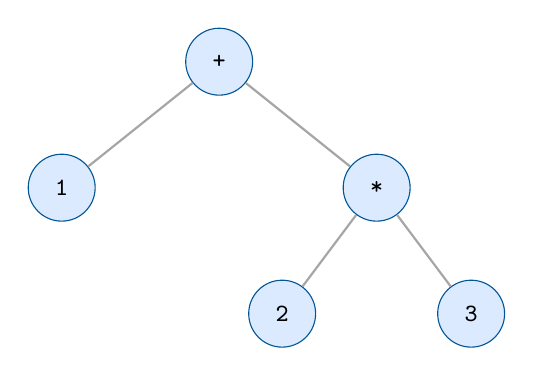
\begin{tikzpicture}[
  nd/.style={circle, draw=NavyBlue, fill=LightBlue,
             minimum size=0.85cm, font=\small\bfseries},
  eg/.style={-, thick, color=gray!70}
]
  \node[nd] (p) at (0,0)      {\texttt{+}};
  \node[nd] (a) at (-2,-1.6)  {\texttt{1}};
  \node[nd] (m) at (2,-1.6)   {\texttt{*}};
  \node[nd] (b) at (0.8,-3.2) {\texttt{2}};
  \node[nd] (c) at (3.2,-3.2) {\texttt{3}};
  \draw[eg] (p)--(a);
  \draw[eg] (p)--(m);
  \draw[eg] (m)--(b);
  \draw[eg] (m)--(c);
\end{tikzpicture}
\end{center}

\subsubsection{节点类设计（C++ 类层次）}

推荐使用\textbf{继承 + 访问者模式}。以下是设计思路（伪代码）：

\begin{lstlisting}[language=C++, caption={AST 节点基类设计思路}]
// 所有节点的抽象基类
struct ASTNode {
    virtual ~ASTNode() = default;
    virtual void accept(ASTVisitor& v) = 0;
};

// 表达式基类
struct Expr : ASTNode {};

// 二元运算：left op right
struct BinaryExpr : Expr {
    std::unique_ptr<Expr> left, right;
    TokenType op;   // PLUS / MINUS / STAR / SLASH ...
    void accept(ASTVisitor& v) override { v.visit(*this); }
};

// 整数字面量
struct NumberLiteral : Expr {
    int value;
    void accept(ASTVisitor& v) override { v.visit(*this); }
};

// 标识符引用（变量名）
struct IdentifierExpr : Expr {
    std::string name;
    void accept(ASTVisitor& v) override { v.visit(*this); }
};

// 语句基类
struct Stmt : ASTNode {};

// if 语句
struct IfStmt : Stmt {
    std::unique_ptr<Expr> condition;
    std::unique_ptr<Stmt> thenBranch;
    std::unique_ptr<Stmt> elseBranch;  // 可为 nullptr
    void accept(ASTVisitor& v) override { v.visit(*this); }
};
\end{lstlisting}

\subsubsection{访问者模式（Visitor Pattern）}

访问者模式使你可以在\textbf{不修改节点类}的前提下，为 AST 添加新操作
（如打印、类型检查、代码生成）：

\begin{lstlisting}[language=C++, caption={访问者接口定义}]
struct ASTVisitor {
    virtual void visit(BinaryExpr& n)     = 0;
    virtual void visit(NumberLiteral& n)  = 0;
    virtual void visit(IdentifierExpr& n) = 0;
    virtual void visit(IfStmt& n)         = 0;
    // ...后续添加更多节点类型时，在此新增虚函数
};

// 实现示例：AST 打印器（调试用）
struct ASTPrinter : ASTVisitor {
    int depth = 0;
    void visit(BinaryExpr& n) override {
        // 打印缩进 + 运算符，然后递归打印左右子树
    }
    // ...
};
\end{lstlisting}

\begin{tipbox}[\texttt{unique\_ptr} 与所有权]
AST 中\textbf{父节点拥有子节点的所有权}。
使用 \texttt{std::unique\_ptr} 来表示，父节点销毁时子节点自动递归销毁，
彻底杜绝内存泄漏，无需手动 \texttt{delete}。
\end{tipbox}

% ------------------------------------------------------
\subsection{阶段四：语义分析}
% ------------------------------------------------------

\subsubsection{任务}

语法分析验证代码\textbf{结构}是否合法，语义分析验证代码\textbf{含义}是否合法：

\begin{itemize}[noitemsep]
  \item 变量必须先声明再使用（未声明应报错）
  \item 赋值时右值类型必须与左值兼容（类型检查）
  \item 函数调用参数数量与声明一致（参数检查）
\end{itemize}

\subsubsection{符号表设计}

符号表记录所有标识符的\textbf{名称、类型、作用域层级}等信息。

\begin{lstlisting}[language=C++, caption={符号表结构示意}]
struct Symbol {
    std::string name;
    DataType    type;       // INT, BOOL, FLOAT ...
    int         scopeLevel;
};

class SymbolTable {
    // 用栈模拟作用域嵌套：最内层作用域在栈顶
    std::vector<std::unordered_map<std::string, Symbol>> scopes;
public:
    void    enterScope();              // 遇到 '{' 时调用
    void    exitScope();               // 遇到 '}' 时调用
    void    define(const Symbol& s);
    Symbol* lookup(const std::string& name);
    // lookup 从栈顶向下查找，实现"内层屏蔽外层"
};
\end{lstlisting}

\subsubsection{类型检查}

遍历 AST，对每个表达式推导其类型并验证操作数兼容性：

\begin{center}
\renewcommand{\arraystretch}{1.3}
\begin{tabular}{ccc}
\toprule
\textbf{操作}      & \textbf{合法性} & \textbf{结果类型} \\
\midrule
\texttt{int + int}  & 合法 & \texttt{int} \\
\texttt{int < int}  & 合法 & \texttt{bool} \\
\texttt{int + bool} & 非法（报错） & -- \\
\texttt{int = bool} & 非法（报错） & -- \\
\bottomrule
\end{tabular}
\end{center}

% ------------------------------------------------------
\subsection{阶段五：中间代码生成（IR）}
% ------------------------------------------------------

\subsubsection{为什么需要中间表示}

直接从 AST 生成目标代码不便于优化。IR（Intermediate Representation）
介于 AST 和目标代码之间，是\textbf{方便进行各种优化分析}的统一表示形式。

\subsubsection{三地址码（Three-Address Code）}

每条指令最多含\textbf{三个地址}（两操作数、一结果）：

\begin{lstlisting}[caption={三地址码指令类型示例}]
x = y op z      // 二元运算（加减乘除、比较）
x = op y        // 一元运算（负号、逻辑非）
x = y           // 赋值/复制
goto L          // 无条件跳转
if x goto L     // 条件跳转
call f, n       // 函数调用（n 为参数数量）
\end{lstlisting}

\textbf{生成思路}：对 AST 进行\textbf{后序遍历}（先处理子树，再处理根节点），
每处理一个节点就生成对应指令，并用临时变量 \texttt{t1}、\texttt{t2}...
存储中间结果。

以 \texttt{if (x > 0) y = 1; else y = -1;} 为例：

\begin{lstlisting}[caption={if-else 语句的三地址码生成示例}]
    t1 = x > 0
    if t1 == false goto L_ELSE
    y = 1
    goto L_END
L_ELSE:
    t2 = -1
    y = t2
L_END:
\end{lstlisting}

\subsubsection{DAG（有向无环图）}

DAG（Directed Acyclic Graph）允许多个节点\textbf{共享相同的子树}，
从而天然消除重复计算。

考虑 \texttt{a = (b + c) + (b + c)}，AST 中 \texttt{b+c} 出现两次，
而 DAG 中根节点的两条边指向\textbf{同一个} \texttt{b+c} 节点：

\begin{center}
\begin{tikzpicture}[
  nd/.style={circle, draw=NavyBlue, fill=LightBlue,
             minimum size=0.8cm, font=\small\bfseries},
  eg/.style={-, thick, color=gray!70}
]
  % ---- AST（左侧）----
  \begin{scope}[xshift=-5cm]
    \node[font=\bfseries\small] at (0, 1.2) {AST（有冗余）};
    \node[nd] (r1) at (0,0)       {\texttt{+}};
    \node[nd] (l1) at (-1.6,-1.5) {\texttt{+}};
    \node[nd] (r2) at (1.6,-1.5)  {\texttt{+}};
    \node[nd] (b1) at (-2.4,-3)   {\texttt{b}};
    \node[nd] (c1) at (-0.8,-3)   {\texttt{c}};
    \node[nd] (b2) at (0.8,-3)    {\texttt{b}};
    \node[nd] (c2) at (2.4,-3)    {\texttt{c}};
    \draw[eg] (r1)--(l1); \draw[eg] (r1)--(r2);
    \draw[eg] (l1)--(b1); \draw[eg] (l1)--(c1);
    \draw[eg] (r2)--(b2); \draw[eg] (r2)--(c2);
  \end{scope}

  % ---- DAG（右侧）----
  \begin{scope}[xshift=3.5cm]
    \node[font=\bfseries\small] at (0, 1.2) {DAG（共享子节点）};
    \node[nd] (root) at (0,0)      {\texttt{+}};
    \node[nd] (add)  at (0,-1.8)   {\texttt{+}};
    \node[nd] (b)    at (-1.5,-3.4){\texttt{b}};
    \node[nd] (c)    at (1.5,-3.4) {\texttt{c}};
    % 根节点的两条边都指向同一个 add 节点（用弯曲边表示）
    \draw[eg] (root) to[out=215, in=110] (add);
    \draw[eg] (root) to[out=325, in=70]  (add);
    \draw[eg] (add)--(b); \draw[eg] (add)--(c);
  \end{scope}
\end{tikzpicture}
\end{center}

\begin{tipbox}[DAG 构建算法核心]
维护一个\textbf{哈希表}，键为 ``运算符 + 左操作数ID + 右操作数ID''。
创建新节点前先查表：若已存在相同节点，直接返回已有 ID（复用），
否则创建新节点并插入表。
这就是\textbf{公共子表达式消除（CSE）}的本质。
\end{tipbox}

% ------------------------------------------------------
\subsection{阶段六：代码生成}
% ------------------------------------------------------

\subsubsection{目标选择（由易到难）}

\begin{enumerate}
  \item \textbf{解释执行三地址码}（最简单，强烈推荐入门）：
        用 C++ 模拟一个虚拟机，直接执行三地址码指令，
        可验证编译器前几阶段的正确性。
  \item \textbf{生成 LLVM IR}（推荐进阶）：
        调用 LLVM C++ API，由 LLVM 负责后端优化和平台汇编生成。
  \item \textbf{生成 x86-64 汇编}（最复杂）：
        直接输出 \texttt{.asm} 文件，需要了解寄存器分配等底层知识。
\end{enumerate}

\begin{warnbox}[关于寄存器分配]
真实的寄存器分配（图着色算法）相当复杂。对于大学生项目，
可以使用\textbf{简化策略：将所有临时变量存放在栈帧上}
（通过 \texttt{mov} 指令存取内存），性能不高但实现简单、功能完全正确。
等功能稳定后再考虑优化寄存器使用策略。
\end{warnbox}

% =======================================================
\section{完整构建步骤}
% =======================================================

\subsection{开发环境准备}

\begin{enumerate}
  \item \textbf{安装 C++ 编译器}：
    \begin{itemize}[noitemsep]
      \item Windows：安装 MinGW-w64，或 Visual Studio（含 MSVC）
      \item Linux：\texttt{sudo apt install build-essential cmake}
      \item macOS：\texttt{xcode-select -{}-install}
    \end{itemize}
  \item \textbf{安装 CMake 3.15+}：从 \href{https://cmake.org/download/}{cmake.org} 下载
  \item \textbf{配置编辑器}：VS Code + C/C++ 扩展 + CMake Tools 扩展
  \item （可选）\textbf{安装 Google Test}：通过 vcpkg 执行
        \texttt{vcpkg install gtest}
\end{enumerate}

\subsection{推荐开发顺序}

\begin{keybox}[按此顺序开发，不容易迷失方向]
\begin{enumerate}
  \item \textbf{词法分析器}：最容易入手，先让 \texttt{"1 + 2"} 正确输出 Token 序列
  \item \textbf{语法分析器 + AST}：实现表达式解析，能打印 AST 的树形结构
  \item \textbf{语义分析}：加入符号表，能检测未声明变量和类型不匹配
  \item \textbf{解释执行（可选）}：直接遍历 AST 求值，验证前三阶段正确性
  \item \textbf{IR 生成}：将 AST 转换为三地址码
  \item \textbf{基础优化}：在 IR 上做常量折叠等简单优化
  \item \textbf{代码生成}：解释执行 IR 或输出目标代码
\end{enumerate}
\end{keybox}

\subsection{增量验证策略}

每完成一个阶段，立即用简单案例验证正确性，不要等到最后才测试：

\begin{center}
\renewcommand{\arraystretch}{1.4}
\begin{tabular}{cl}
\toprule
\textbf{阶段} & \textbf{验证方式} \\
\midrule
词法 & 对 \texttt{"x = 1 + 2 * 3;"} 打印出正确的 Token 序列 \\
语法 & 对上述输入打印出正确的 AST 树形 \\
语义 & 对未声明变量 \texttt{y} 报错；对 \texttt{int x = true;} 报类型错误 \\
IR   & 对 \texttt{"a = 1 + 2 * 3;"} 生成正确的三地址码 \\
代码 & 对 \texttt{"int a=1; int b=2; print(a+b);"} 输出 \texttt{3} \\
\bottomrule
\end{tabular}
\end{center}

% =======================================================
\section{性能优化建议}
% =======================================================

\begin{warnbox}[优化的黄金原则]
\textbf{先让编译器正确运行，再做优化！}
优化应在 IR 阶段以独立的 ``pass'' 形式实现，不要在 AST 阶段修改树结构。
每个 pass 只做一件事，便于单独测试和调试。
\end{warnbox}

% ------------------------------------------------------
\subsection{常量折叠（Constant Folding）}
% ------------------------------------------------------

若表达式的所有操作数在\textbf{编译期都是常量}，则直接计算结果，
不生成任何运行时计算指令。

\begin{center}
\renewcommand{\arraystretch}{1.3}
\begin{tabular}{ccc}
\toprule
\textbf{优化前} & & \textbf{优化后} \\
\midrule
\texttt{1 + 2}           & $\Rightarrow$ & \texttt{3} \\
\texttt{3 * 4 - 2}       & $\Rightarrow$ & \texttt{10} \\
\texttt{2 * 0}           & $\Rightarrow$ & \texttt{0} \\
\texttt{true \&\& false} & $\Rightarrow$ & \texttt{false} \\
\bottomrule
\end{tabular}
\end{center}

\textbf{实现思路}：在生成 IR 时，若 \texttt{BinaryExpr} 的两个子节点均为字面量，
则在编译期直接计算结果，返回一个新的字面量节点，不生成三地址码指令。

% ------------------------------------------------------
\subsection{代数化简（Algebraic Simplification）}
% ------------------------------------------------------

利用基本数学性质化简表达式，实现简单但收益明显：

\begin{center}
\renewcommand{\arraystretch}{1.3}
\begin{tabular}{ccc}
\toprule
\textbf{原表达式} & \textbf{规则} & \textbf{化简结果} \\
\midrule
\texttt{x + 0}    & 加法单位元   & \texttt{x} \\
\texttt{x * 1}    & 乘法单位元   & \texttt{x} \\
\texttt{x * 0}    & 零乘法则     & \texttt{0} \\
\texttt{x - x}    & 自身相减     & \texttt{0} \\
\texttt{x / x}    & 自身相除     & \texttt{1}（排除 \texttt{x=0}） \\
\texttt{-(-x)}    & 双重否定     & \texttt{x} \\
\texttt{x + (-y)} & 加负等于减   & \texttt{x - y} \\
\bottomrule
\end{tabular}
\end{center}

\textbf{实现思路}：在 IR 优化 pass 中，对每条三地址码做模式匹配，
识别并替换符合上述规则的指令。例如，识别 \texttt{x = y + 0} 直接替换为 \texttt{x = y}。

% ------------------------------------------------------
\subsection{负号合并详细示例}
% ------------------------------------------------------

以 \texttt{1 + (-1)} 为例，展示代数化简的完整优化过程：

\begin{lstlisting}[caption={\texttt{1 + (-1)} 的分步优化过程}]
// 源代码
a = 1 + (-1)

// 未优化的三地址码（直接翻译）
t1 = -1          // 一元负号：生成一条指令
t2 = 1 + t1      // 加法：又生成一条指令

// 第一步：代数化简（加负 -> 减法）
//   识别 "x + (-y)" 模式，改写为 "x - y"
t2 = 1 - 1       // 省去了 t1 的计算，少一条指令

// 第二步：常量折叠（两个常量相减）
a = 0            // 直接得到结果，彻底消除运算
\end{lstlisting}

% ------------------------------------------------------
\subsection{公共子表达式消除（CSE）}
% ------------------------------------------------------

若同一个表达式在程序中被计算多次，只计算一次并将结果复用：

\begin{lstlisting}[caption={CSE 优化示例}]
// 优化前的三地址码
t1 = b + c
t2 = b + c      // 与 t1 完全相同，重复计算！
t3 = t1 * t2

// CSE 优化后
t1 = b + c
t3 = t1 * t1    // 复用 t1，省去一次加法
\end{lstlisting}

\textbf{实现思路}：

\begin{itemize}[noitemsep]
  \item \textbf{方法一（推荐）}：基于 DAG 构建（见第4.5节），
        哈希表机制天然支持 CSE
  \item \textbf{方法二}：在三地址码上维护``可用表达式集合''，
        每次生成新指令前查表，若已有相同表达式则复用结果变量名
\end{itemize}

% ------------------------------------------------------
\subsection{死代码消除（Dead Code Elimination）}
% ------------------------------------------------------

删除不可能被执行、或对最终结果没有影响的代码：

\begin{lstlisting}[caption={死代码消除示例}]
// 优化前（if 条件是编译期常量 false）
if (false) {
    x = 100;    // 永远不会执行
}
y = 2;

// 死代码消除后（整个 if 分支被删除）
y = 2;
\end{lstlisting}

\textbf{实现思路}：在常量折叠之后，检查 \texttt{if} 语句的条件是否已经是编译期常量
（\texttt{true}/\texttt{false}），若是则只保留对应分支，丢弃另一分支代码。

% ------------------------------------------------------
\subsection{指令重排（Instruction Reordering）}
% ------------------------------------------------------

在\textbf{不改变程序语义}的前提下，调整指令顺序以减少流水线停顿、
提高 CPU 利用率：

\begin{lstlisting}[caption={指令重排示例（减少数据依赖等待）}]
// 重排前（存在数据依赖导致流水线停顿）
t1 = load a         // 访问内存，有延迟
t2 = t1 + 1         // 必须等 t1 就绪，流水线空转
t3 = load b         // 独立操作，可以提前

// 重排后（t3 的加载与 t1 的加载并行进行）
t3 = load b         // 提前执行，填充流水线空泡
t1 = load a
t2 = t1 + 1         // 此时 t1 已就绪
\end{lstlisting}

\begin{tipbox}[何时可以重排]
两条指令可以交换顺序，当且仅当：
\begin{enumerate}[noitemsep]
  \item 它们之间\textbf{没有数据依赖}（第一条的输出不是第二条的输入）
  \item 没有\textbf{副作用冲突}（如不写同一内存地址）
\end{enumerate}
对大学生项目来说，实现一个简单的``检查两条指令是否读写相同变量''
的判断函数即可满足基本需求。
\end{tipbox}

% =======================================================
\section{实战难点预警}
% =======================================================

\subsection{内存管理}

\begin{keybox}[黄金法则：所有权明确]
在 AST 和 IR 中，\textbf{始终用 \texttt{std::unique\_ptr} 表示所有权}。
禁止裸 \texttt{new}/\texttt{delete}，让 RAII 自动管理生命周期。

\textbf{传递规则}：
\begin{itemize}[noitemsep]
  \item 转移所有权 $\to$ 用 \texttt{std::move(ptr)}
  \item 只是借用，不转移 $\to$ 传 \texttt{T*} 裸指针或 \texttt{const T\&}
\end{itemize}
\end{keybox}

可以用 \texttt{using} 别名减少视觉负担：

\begin{lstlisting}[language=C++, caption={用 using 简化智能指针书写}]
// 在 AST.h 开头定义
template<typename T>
using Ptr = std::unique_ptr<T>;

// 使用时更简洁
Ptr<Expr> left;    // 等同于 std::unique_ptr<Expr> left;
Ptr<Stmt> body;    // 等同于 std::unique_ptr<Stmt> body;
\end{lstlisting}

\subsection{统一错误处理}

设计 \texttt{ErrorHandler} 类，让所有模块通过它报告错误，
而不是直接打印到 \texttt{std::cerr}：

\begin{lstlisting}[language=C++, caption={ErrorHandler 设计思路}]
class ErrorHandler {
    int errorCount   = 0;
    int warningCount = 0;
public:
    void error(int line, int col, const std::string& msg) {
        ++errorCount;
        std::cerr << "error: [第" << line << "行, 第"
                  << col << "列] " << msg << "\n";
    }
    void warning(int line, int col, const std::string& msg);
    bool hasErrors() const { return errorCount > 0; }
};
\end{lstlisting}

好的错误信息示例：

\begin{lstlisting}[caption={错误信息格式参考}]
error:   [第5行, 第10列] 期望 ';' 但遇到了 'if'
error:   [第8行, 第3列]  变量 'x' 未声明即使用
warning: [第3行, 第7列]  变量 'tmp' 已声明但从未使用
\end{lstlisting}

\subsection{常见 Bug 预警}

\begin{warnbox}[这些 Bug 几乎人人都会遇到]
\begin{enumerate}
  \item \textbf{无限循环解析}：递归下降中忘记消耗 Token，导致无限递归直至栈溢出。
        \textit{排查方法}：每次进入解析函数，确保 Token 指针在某处前进了。

  \item \textbf{符号表作用域泄漏}：退出 \texttt{\}} 时忘记调用 \texttt{exitScope()}，
        导致内层局部变量在外层仍然可见。

  \item \textbf{移动后再使用 \texttt{unique\_ptr}}：将 \texttt{unique\_ptr}
        通过 \texttt{std::move()} 传入函数后，原变量变为 \texttt{nullptr}，
        再次解引用会直接崩溃。

  \item \textbf{空 else 分支}：\texttt{if} 不一定有 \texttt{else}，
        在代码生成阶段必须检查 \texttt{elseBranch != nullptr}。

  \item \textbf{左递归死循环}：文法中存在左递归（如 \texttt{expr -> expr '+' expr}）
        会使递归下降解析器无限循环，需改写为右递归或迭代（循环）形式。
\end{enumerate}
\end{warnbox}

\subsection{推荐学习资源}

\begin{itemize}
  \item \textbf{Crafting Interpreters}（Robert Nystrom，免费在线）：
        用 Java/C 从零实现解释器，思路极为清晰，\textbf{强烈推荐作为主要参考}

  \item \textbf{《自制编译器》}（青木峰郎）：
        中文版，适合大学生入门，示例代码清晰易懂

  \item \textbf{《编译原理》}（龙书，Aho 等）：
        权威教材，内容全面，可作为查阅参考

  \item \textbf{LLVM Kaleidoscope Tutorial}：\\
        \href{https://llvm.org/docs/tutorial/}{https://llvm.org/docs/tutorial/}\\
        从零用 LLVM API 实现一门完整语言，是学习 LLVM 后端的最佳起点
\end{itemize}

% =======================================================
\section{总结}
% =======================================================

构建编译器是计算机科学中最有成就感的项目之一。牢记以下要点：

\begin{enumerate}
  \item \textbf{一步一步来}：先跑通 \texttt{1 + 2}，再扩展 \texttt{if}/\texttt{while}，
        不要一开始就沉迷于复杂优化
  \item \textbf{打印中间结果}：词法阶段打印 Token，语法阶段打印 AST，
        这是定位 bug 最快的方法
  \item \textbf{测试先行}：每完成一个模块立即写测试，不要等到集成阶段再测
  \item \textbf{用好工具}：CMake 管理构建，GDB 调试崩溃，Git 保存进度
  \item \textbf{不怕出错}：编译器的错误信息是你的朋友，认真阅读每一条
\end{enumerate}

\vspace{1.5cm}
\begin{center}
  \Large\bfseries\color{NavyBlue} 祝你的编译器大作业顺利完成！
\end{center}

\end{document}
